\documentclass[letterpaper,9pt,twocolumn,twoside,]{pinp}

%% Some pieces required from the pandoc template
\providecommand{\tightlist}{%
  \setlength{\itemsep}{0pt}\setlength{\parskip}{0pt}}

% Use the lineno option to display guide line numbers if required.
% Note that the use of elements such as single-column equations
% may affect the guide line number alignment.

\usepackage[T1]{fontenc}
\usepackage[utf8]{inputenc}

% pinp change: the geometry package layout settings need to be set here, not in pinp.cls
\geometry{layoutsize={0.95588\paperwidth,0.98864\paperheight},%
  layouthoffset=0.02206\paperwidth, layoutvoffset=0.00568\paperheight}

\definecolor{pinpblue}{HTML}{185FAF}  % imagecolorpicker on blue for new R logo
\definecolor{pnasbluetext}{RGB}{101,0,0} %



\title{Optimizing Candy Land ``House Rules'': Reducing parental
toddler-bedtime-routine-induced distress}

\author[a,b]{Mathew V Kiang}

  \affil[a]{Instructor, Department of Epidemiology and Population Health, Stanford
University}
  \affil[b]{Fellow, Harvard FXB Center for Health and Human Rights, Harvard
University}

\setcounter{secnumdepth}{0}

% Please give the surname of the lead author for the running footer
\leadauthor{Optimizing Candy Land ``House Rules''}

% Keywords are not mandatory, but authors are strongly encouraged to provide them. If provided, please include two to five keywords, separated by the pipe symbol, e.g:
 \keywords{  mental health |  child development |  monte carlo simulation |  game theory  }  

\begin{abstract}
Children are wonderful. However, there are situations in which parents
must minimize the amount of time spent on an activity while maximizing a
child's enjoyment of the activity. Here, we analyze the problem of a
bedtime routine that involves playing the game Candy Land with a toddler
who does not take kindly to losing. We examine variants of the rule sets
to create ``house rules'' that optimize the probability of the toddler
winning while minimizing the amount of time playing. We find that
adopting a ``Youngest Forward-Only'' set significantly improves the
probability of the toddler winning with minimal impact on duration of
play. A ``All Best Choice'' set produces the shortest games but does not
substantially improve the winning probability of the toddler. Lastly, a
``Youngest Best Choice'' set nearly ensures toddler victory while still
providing the same or shorter game duration as the Standard set of
rules.
\end{abstract}

\dates{This version was compiled on \today} 

% initially we use doi so keep for backwards compatibility
% new name is doi_footer
\doifooter{\url{http://github.com/mkiang/optimizing_candyland}}

\pinpfootercontents{Brief Report}

\begin{document}

% Optional adjustment to line up main text (after abstract) of first page with line numbers, when using both lineno and twocolumn options.
% You should only change this length when you've finalised the article contents.
\verticaladjustment{-2pt}

\maketitle
\thispagestyle{firststyle}
\ifthenelse{\boolean{shortarticle}}{\ifthenelse{\boolean{singlecolumn}}{\abscontentformatted}{\abscontent}}{}

% If your first paragraph (i.e. with the \dropcap) contains a list environment (quote, quotation, theorem, definition, enumerate, itemize...), the line after the list may have some extra indentation. If this is the case, add \parshape=0 to the end of the list environment.


\hypertarget{introduction}{%
\section{Introduction}\label{introduction}}

Bedtime routines are a critical aspect of daily life for millions of
American families. Not only do good bedtime routines ensure a
well-rested child, they also play an important role in preserving the
mental health of parents. Often, bedtime routines consists of
screen-time-minimizing activities such as solving puzzles, building
couch forts, or playing board games.

Toddlers do not have fully developed brains. As such, their sense of
fairness is rarely accurate. In addition, toddlers may be
hyper-competitive, believing they deserve to win every game they play.
While there is a time and place for parents, educators, and other adults
to help elucidate these matters as children grow --- bedtime is not it.
For millions of parents, the only single, overriding priority during
bedtime routines is to get the toddler into bed as quickly, quietly, and
calmly as possible.

Here, we explore the statistical properties of Candy Land, a game
frequently played during bedtime routines. We discuss the practical
implications of these properties and explore variations of the game
rules in relation to two objectives: (1) maximize the probability of the
toddler winning while (2) minimize the amount of time playing.

\hypertarget{about-candy-land}{%
\section{About Candy Land}\label{about-candy-land}}

Candy Land, created in 1949, is a simple, non-strategic racing game. It
is a favorite among toddlers because it requires only minimal counting
ability (up to two) and rudimentary recognition of six colors and eight
candies. The components of Candy Land consists of a board, four player
markers, and a deck of 64 cards.

\begin{figure}

{\centering 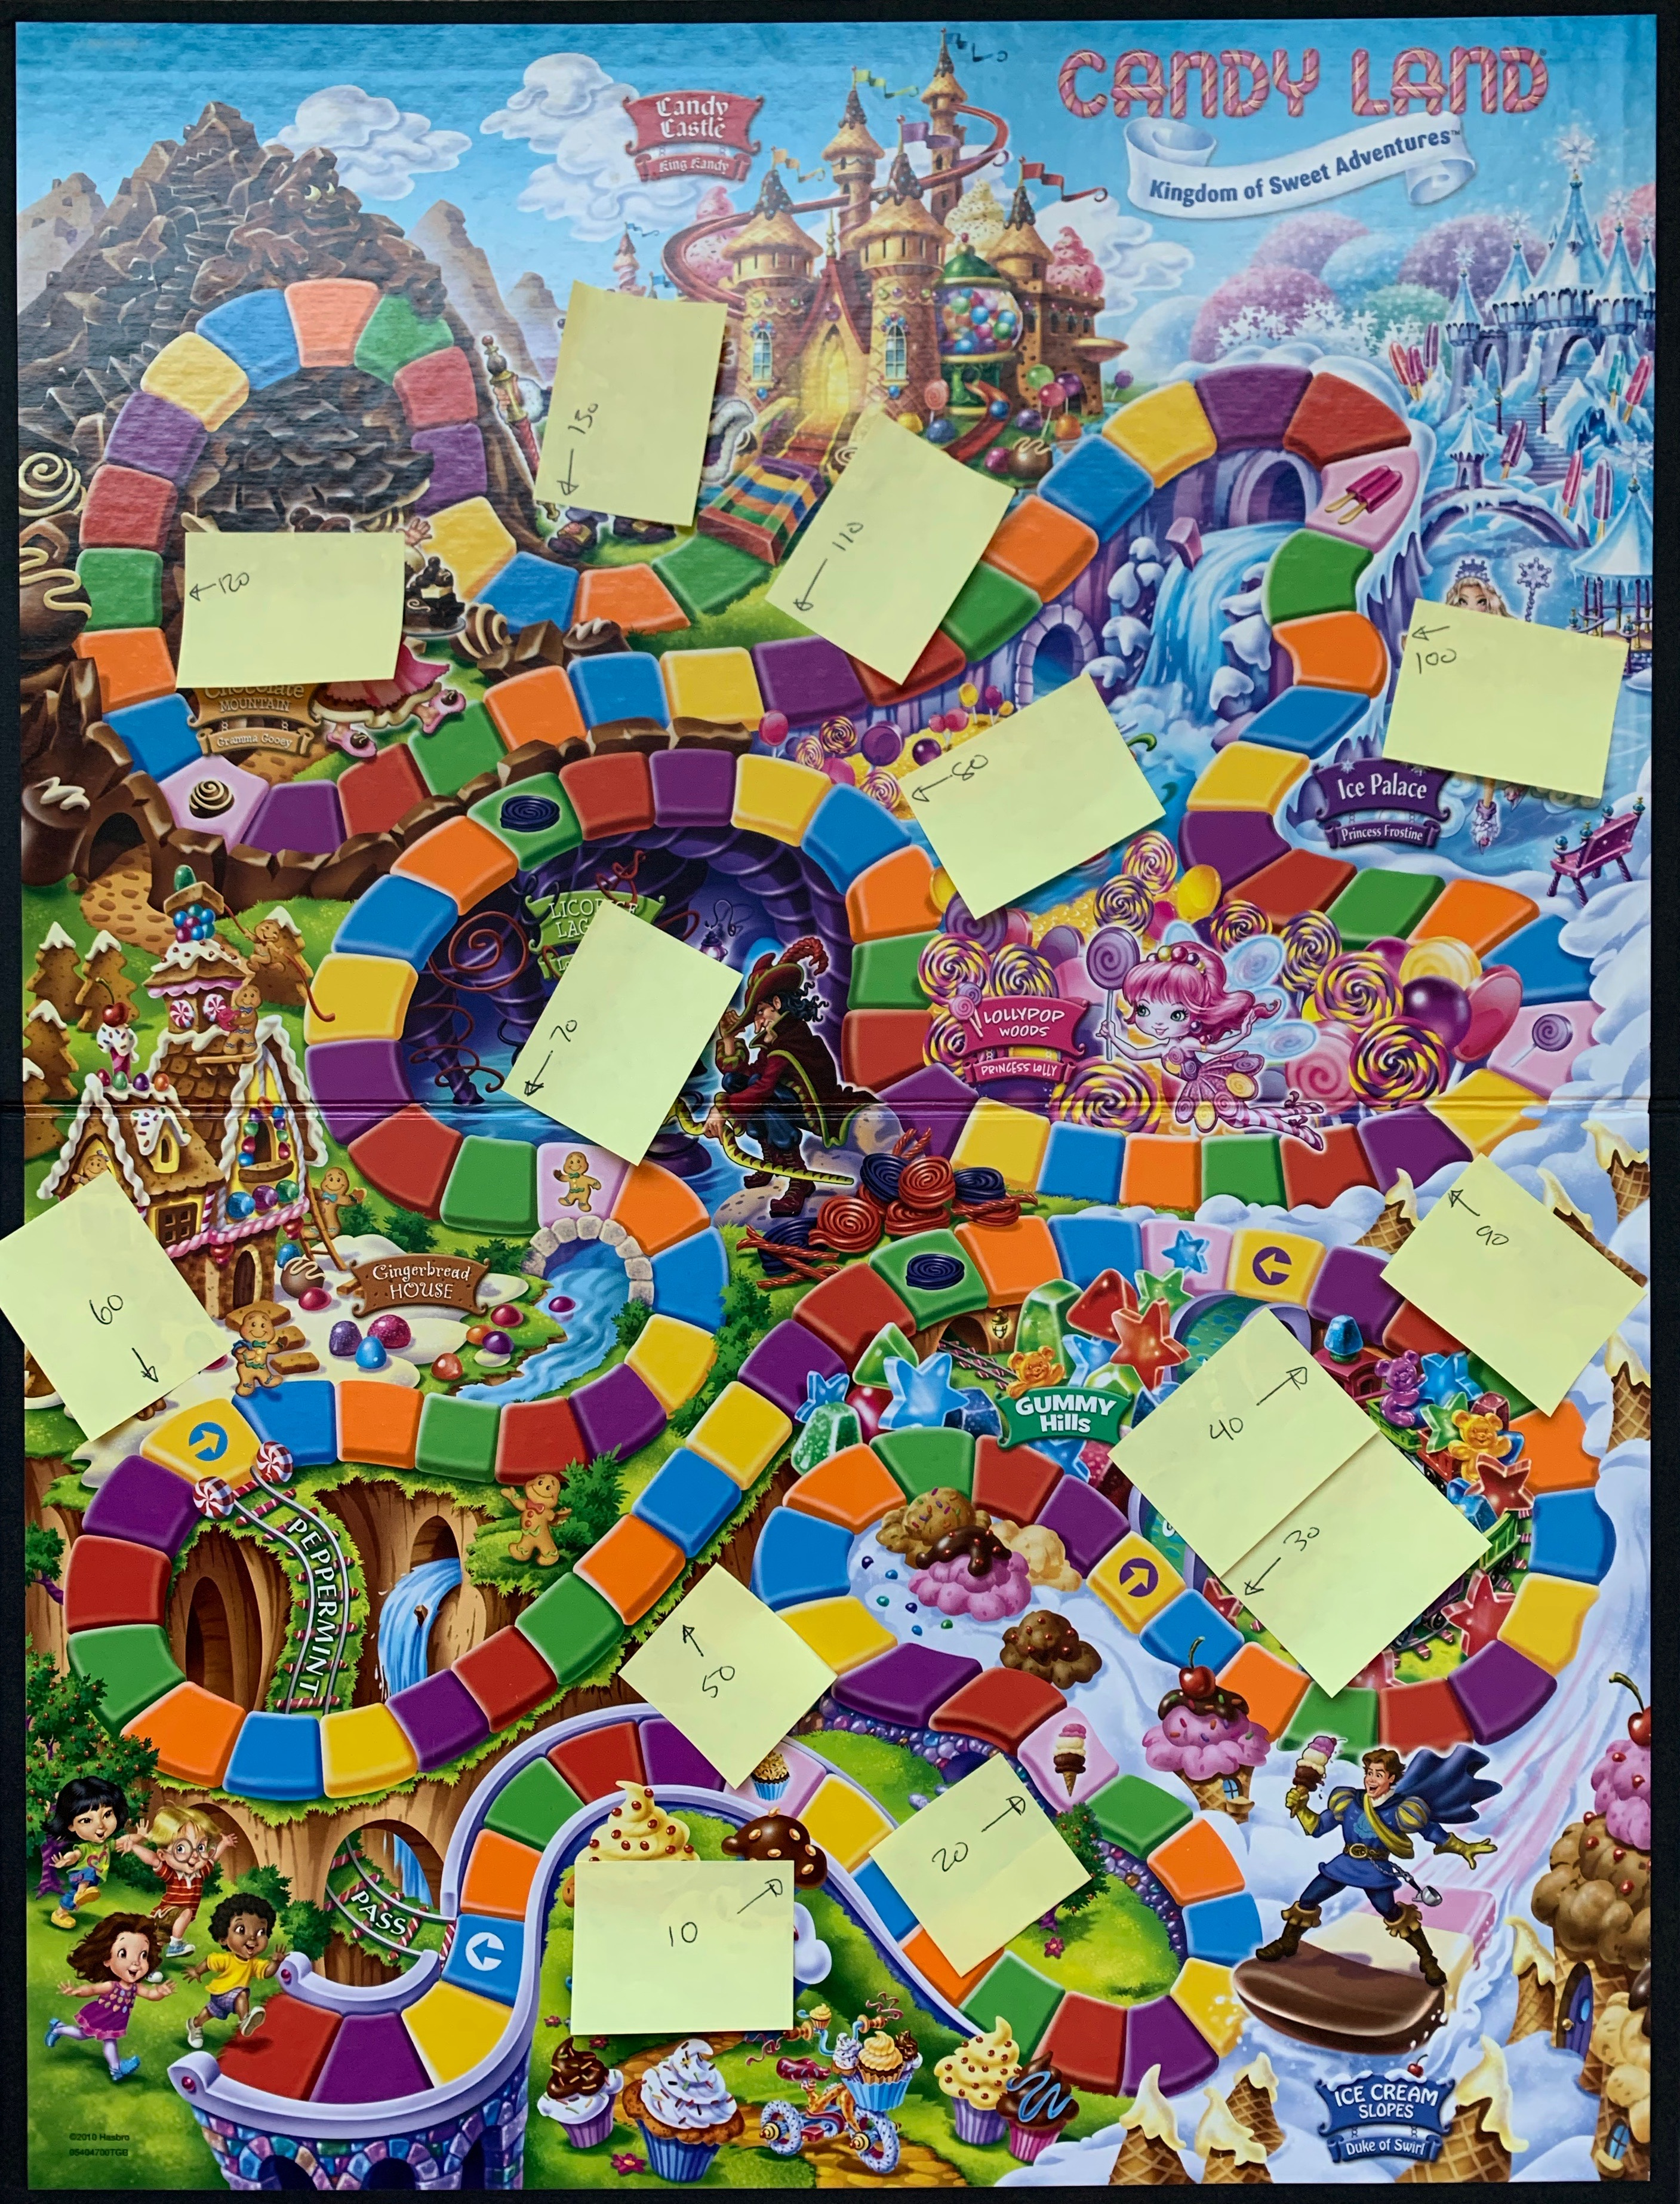
\includegraphics[width=0.75\linewidth]{/Users/mvk/Dropbox/Projects_Ideas/candyland_analysis/data_raw/board_numbered} 

}

\caption{Candy Land board game with notes enumerating every ten spaces. Play begins in the lower left and continues along the paths until a single player reaches the top middle castle.}\label{fig:unnamed-chunk-3}
\end{figure}

Fig. 1 shows the standard Candy Land board with every tenth space
enumerated by a field researcher's hand-written (post-it) notes. On the
board, play begins in the lower left corner and terminates in the top
middle castle. The board follows an approximately repeating pattern of
red, purple, yellow, blue, orange, and green, with special pink squares
interspersed throughout for a total of 132 spaces. Two green squares
have licorice icons and two squares ``teleport'' players forward (but
never backwards).

\begin{figure}

{\centering 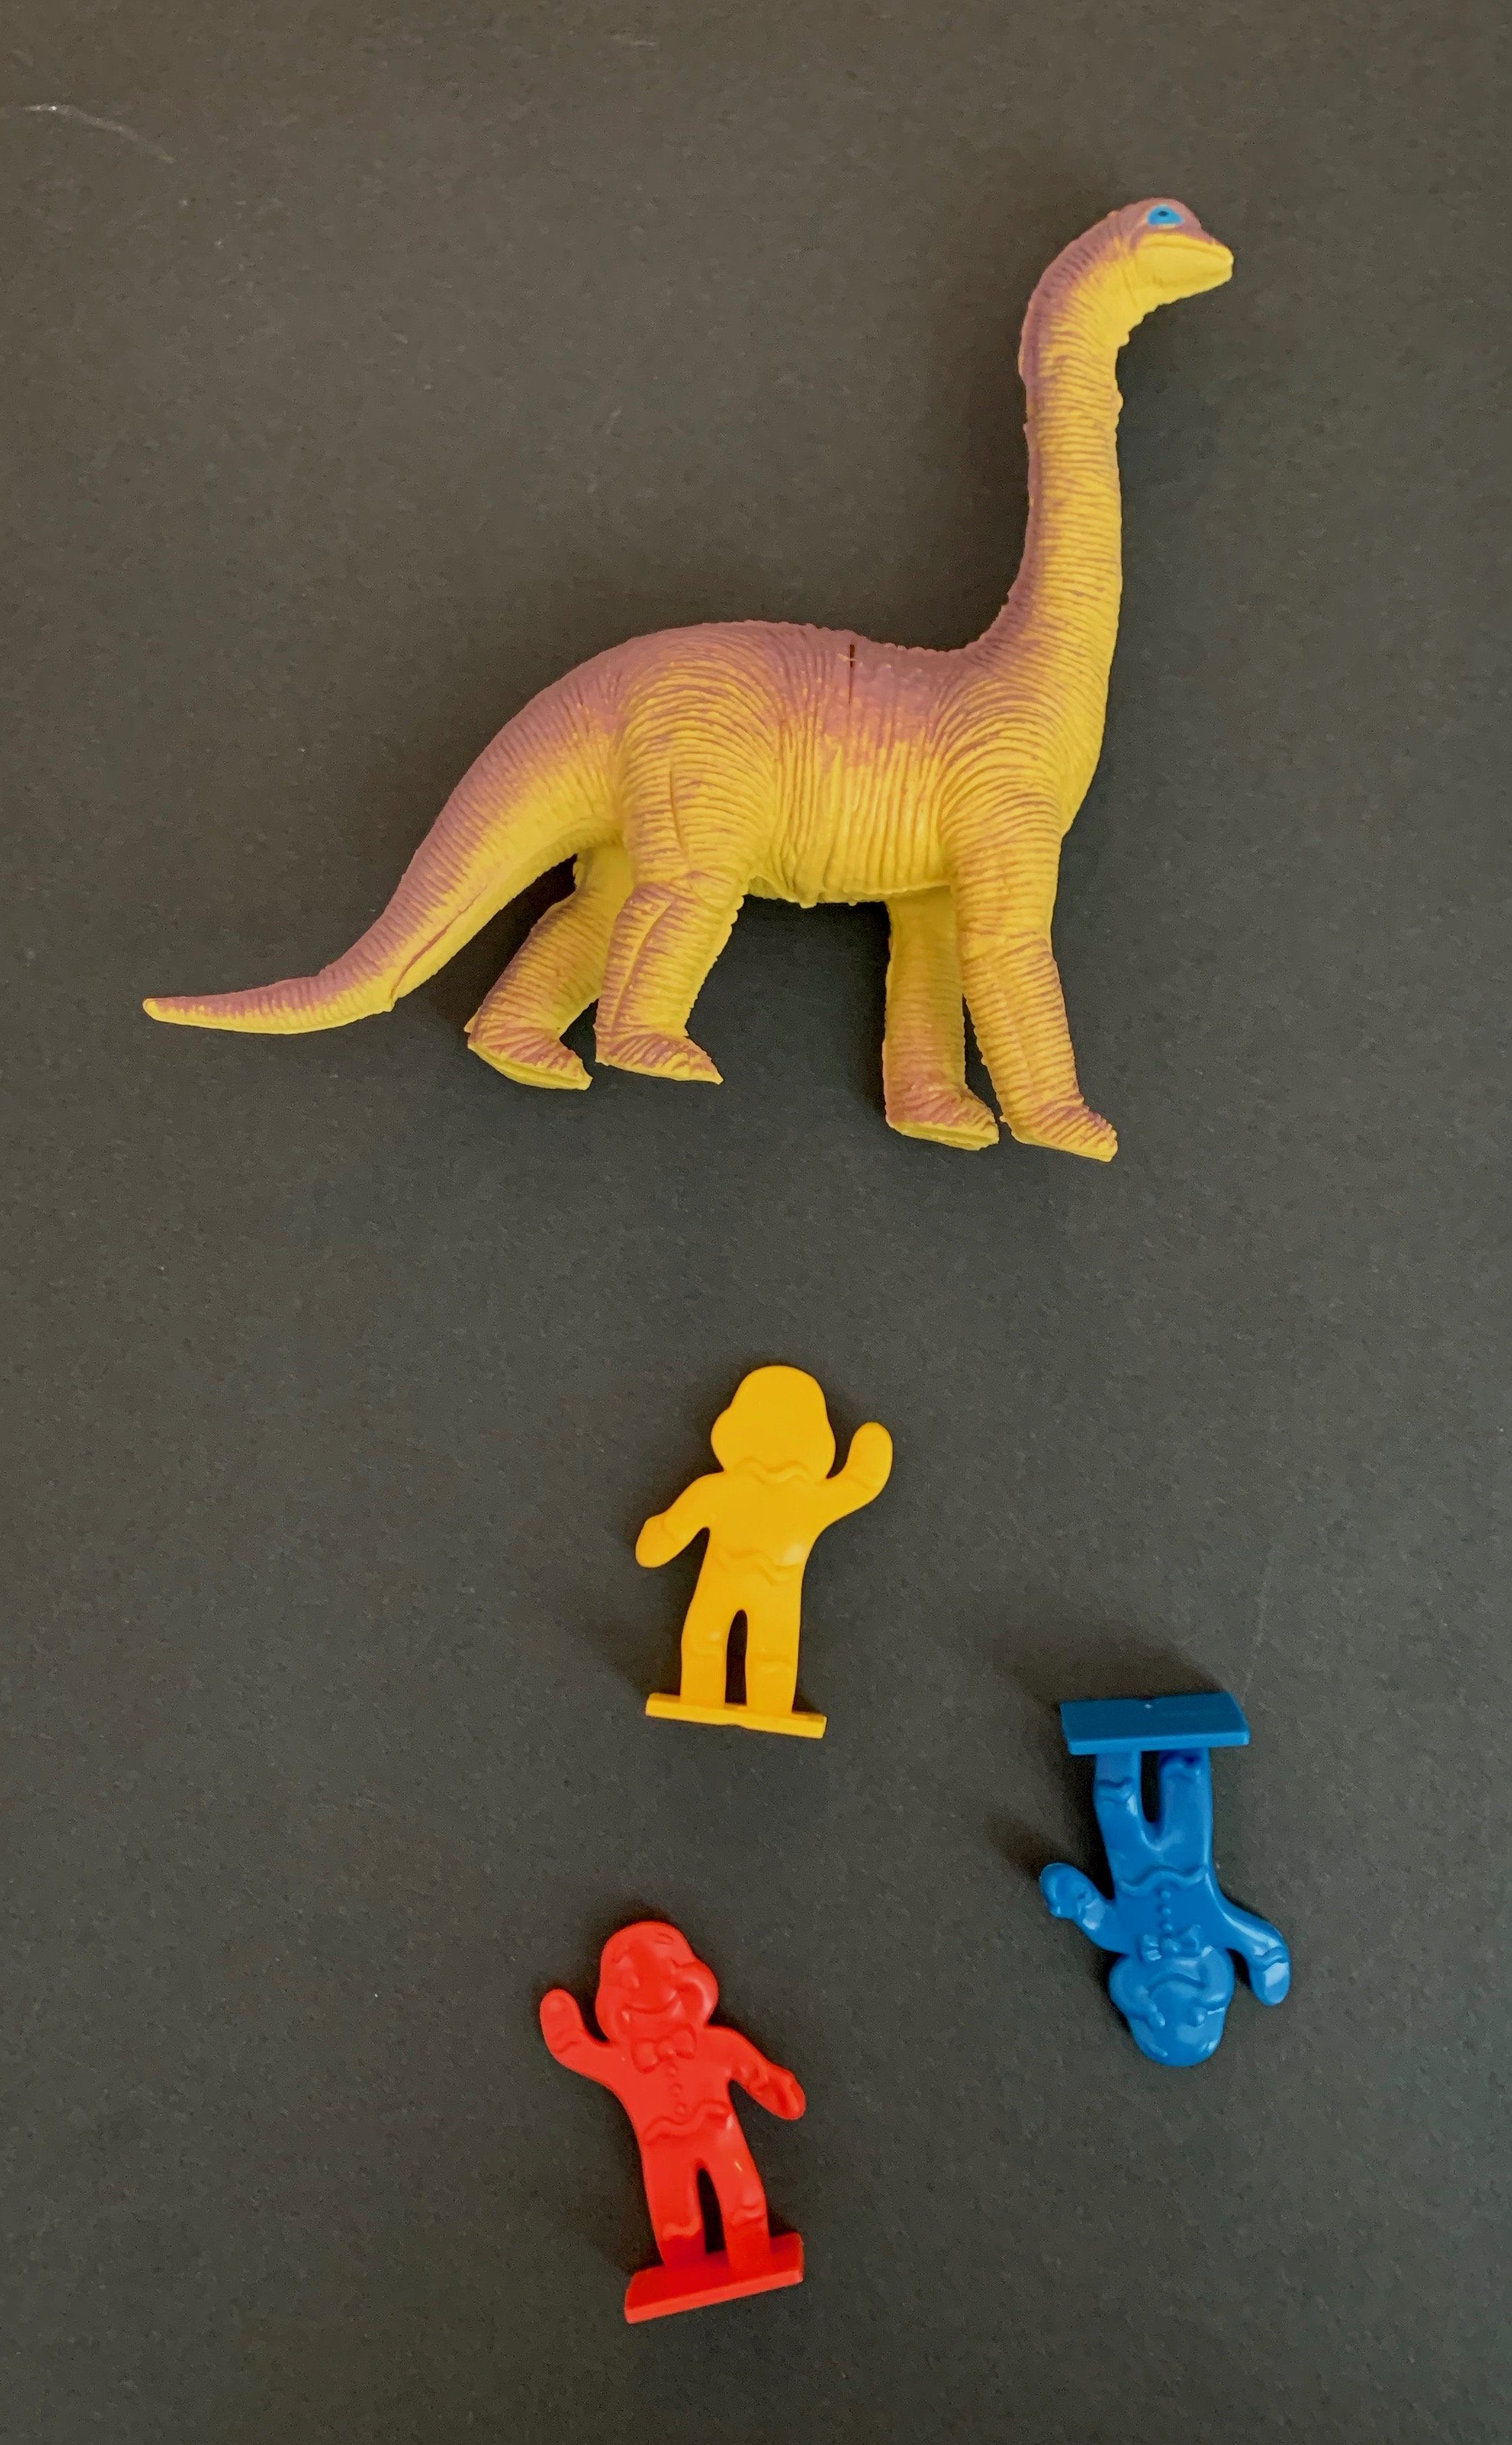
\includegraphics[width=1\linewidth]{/Users/mvk/Dropbox/Projects_Ideas/candyland_analysis/data_raw/player_pieces} 

}

\caption{Player markers. A fourth traditional marker has been replaced by the nearest appropriate item.}\label{fig:unnamed-chunk-4}
\end{figure}

Each player is represented by a marker (Fig. 2) --- the standard fourth
marker in this specific specimen was lost to the ravages of toddler-time
and replaced by a dinosaur. The accompany deck consisting of 64 cards
(Fig. 3). Cards can be single-color, double-color, or one of seven pink
specialty candy locations (see For any given bedtime routine, the ideal
rule set will vary. Text S1).

\begin{figure}

{\centering 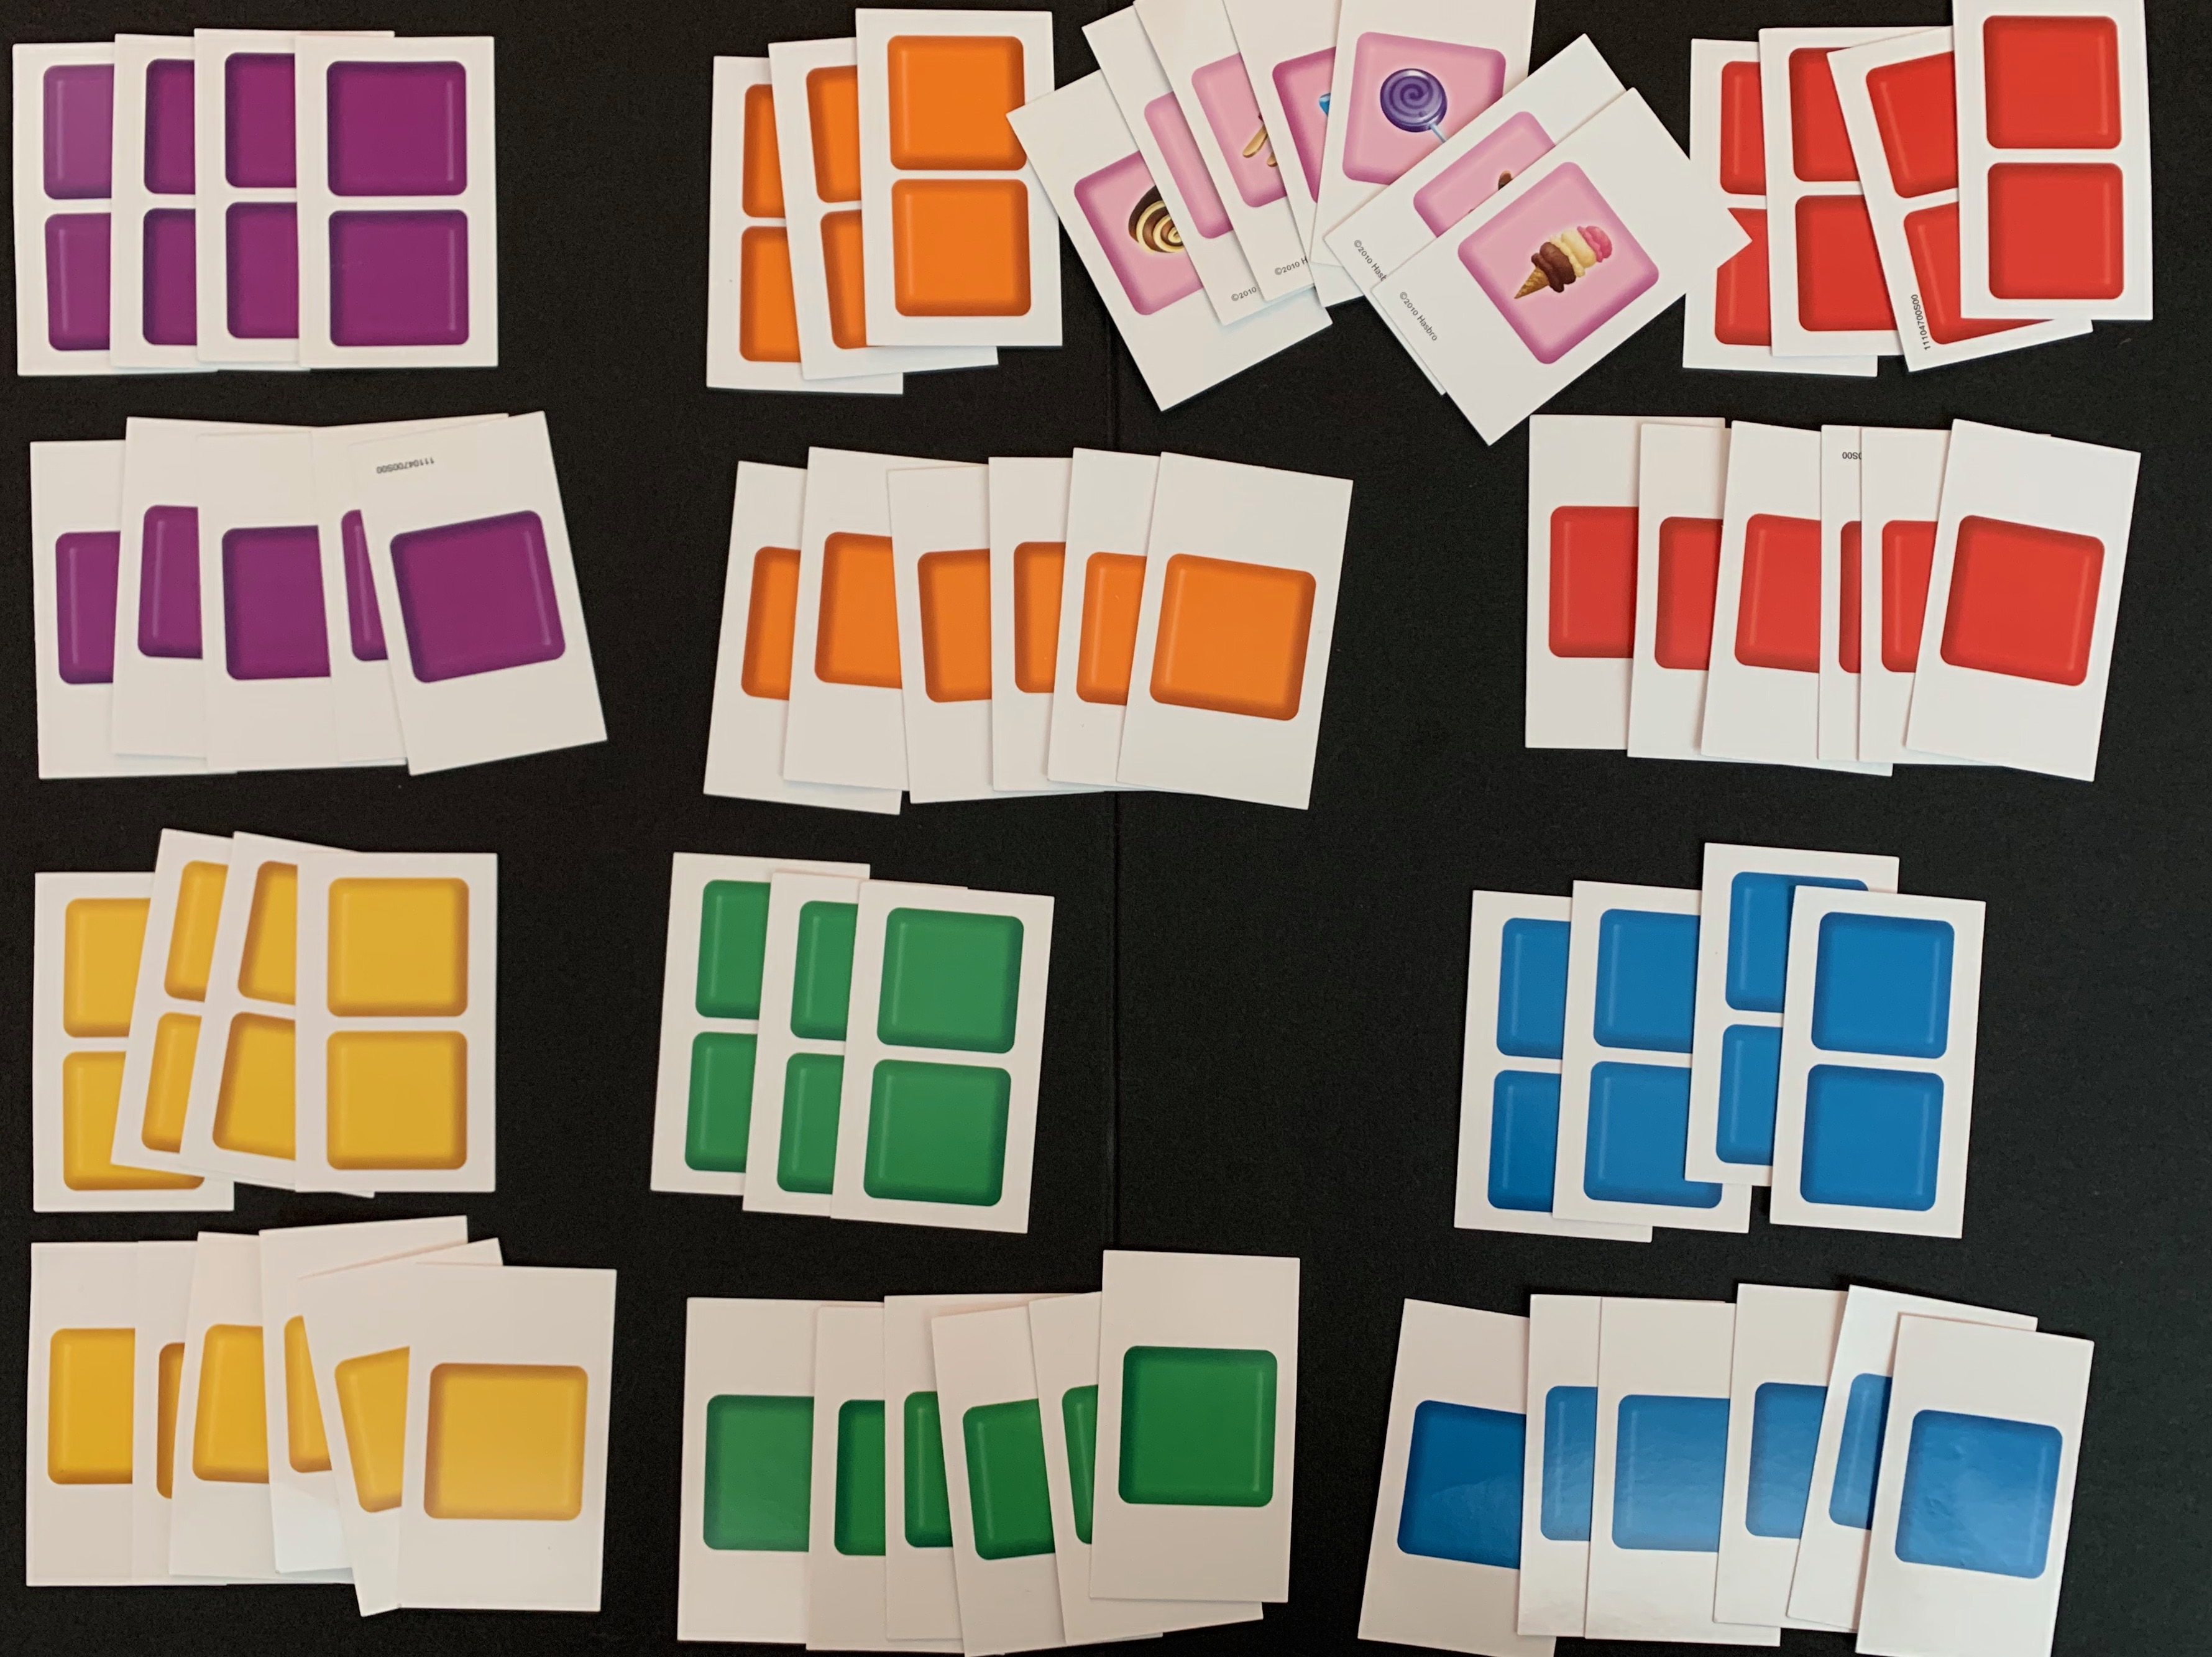
\includegraphics[width=1\linewidth]{/Users/mvk/Dropbox/Projects_Ideas/candyland_analysis/data_raw/cards_sorted} 

}

\caption{The deck is composed of 64 cards which can be single-color, double-color, or special candy location cards.}\label{fig:unnamed-chunk-5}
\end{figure}

\hypertarget{the-rules-of-candy-land}{%
\subsection{The Rules of Candy Land}\label{the-rules-of-candy-land}}

The \textbf{Standard} set of rules are:

\begin{enumerate}
\def\labelenumi{\arabic{enumi}.}
\tightlist
\item
  Each player (starting with the youngest) takes turns, drawing a card.
\item
  If a card has one red, purple, yellow, blue, orange, or green square,
  the player moves \textbf{forward} to the nearest square of
  corresponding color.
\item
  If a card has two red, purple, yellow, blue, orange, or green squares,
  the player moves \textbf{forward} to the second nearest square of
  corresponding color.
\item
  If the card has a candy icon, the player moves \textbf{forward} or
  \textbf{backward} to the corresponding square.
\item
  If a player lands on a green licorice square, they lose a turn.
\item
  If a player lands on Peppermint Pass or Gumdrop Pass, they proceed on
  the indicated path to the corresponding square.
\end{enumerate}

In addition, the instructions provide two variations of the Standard set
of rules.

First, called the ``\textbf{Youngest Forward-Only}'' set, all Standard
rules apply except Player 1 (the youngest player) never moves backwards.
If Player 1 draws a pink card and the location is backwards, they do not
move.

Second, in a Choice set, all players draw two cards and choose one card
before moving. Here, we provide two variations of the Choice set called
the ``All Best Choice'' set and the ``Youngest Best Choice'' set. In the
\textbf{All Best Choice} set, every play draws two cards and always
picks the card that advances their marker the furthest. In the
\textbf{Youngest Best Choice} set, all players draw two cards and the
youngest player always selects the card that advances their marker the
furthers (with help from parents, if necessary); however, all other
players select the card that advances their marker the nearest.

\hypertarget{results}{%
\section{Results}\label{results}}

For each of the four rule sets described above, we ran 100,000 Candy
Land simulations using \texttt{R\ 4.0.2} (see \textbf{Methods} for
details). Each simulated game features three players and, in accordance
to Candy Land regulations, Player 1 is always the youngest player.

Below, we present the statistical properties of Candy Land. We first
discuss the probability of Player 1 winning (Objective 1), then the
distribution of game duration (Objective 2). We then discuss both
Objective 1 and Objective 2 simultaneously. Lastly, we discuss patterns
of mobility in Candy Land.

\hypertarget{player-1-wins-nearly-all-games-under-the-youngest-best-choice-set}{%
\subsection{Player 1 wins nearly all games under the Youngest Best
Choice
set}\label{player-1-wins-nearly-all-games-under-the-youngest-best-choice-set}}

In Fig. \ref{fig:p_win_props}, we plot the proportion of games won by
each player in each rule set. We note that even in the Standard set,
Player 1 has a first-move advantage winning slightly more games than
Player 2 who in turn wins slightly more games than Player 3 (34.7\% vs
33.3\% vs 31.9\%). As expected, the Standard set and the All Best Choice
set yield similar win proportions because they do not restrict the
movement of Player 1. Conversely, Player 1 wins nearly half of all games
in the Youngest Forward-Only set (47\%) and over 99.5\% of all games in
the Youngest Best Choice set. In 100,000 simulated games, Players 2 and
3 won only 96 and 112 Youngest Best Choice games, respectively.

\begin{figure}
  \begin{center}
    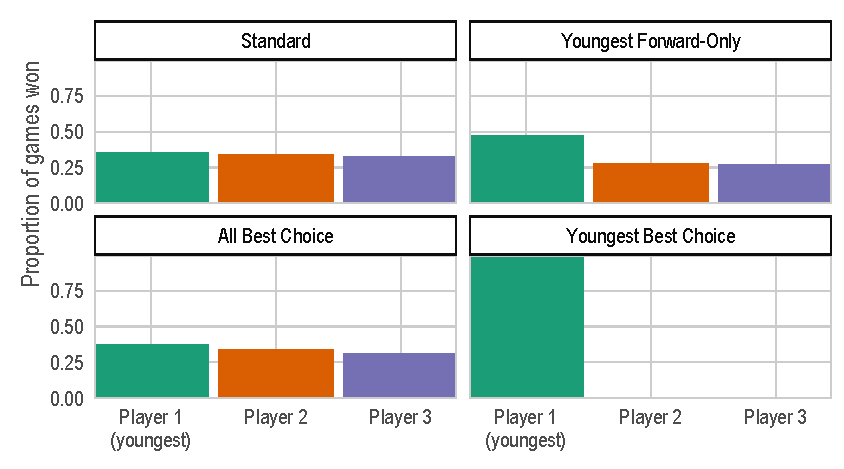
\includegraphics[width=3in]{./../../plots/p_win_props.pdf}
    \caption{Proportion (y-axis) of games won by each player (x-axis) by rule set (facets).}
    \label{fig:p_win_props}
  \end{center}
\end{figure}

\hypertarget{game-duration-is-shortest-under-the-all-best-choice-set}{%
\subsection{Game duration is shortest under the All Best Choice
set}\label{game-duration-is-shortest-under-the-all-best-choice-set}}

In Fig. \ref{fig:p_winning_dist}, we show the duration of games (as
number of moves required by the winning player) under each rule set. All
variants reduced the number of moves required to win relative to the
Standard set. In the Standard set, the winning player required an
average (SD) of 13.0 (5.82) moves before winning compared to 12.0 (4.80)
moves in the Youngest Forward-Only set. The All Best Choice (mean: 7.0;
SD: 2.21) and Youngest Best Choice (mean: 10.7; SD: 3.93) sets reduced
variation while also lowering game time.

\begin{figure}
  \begin{center}
    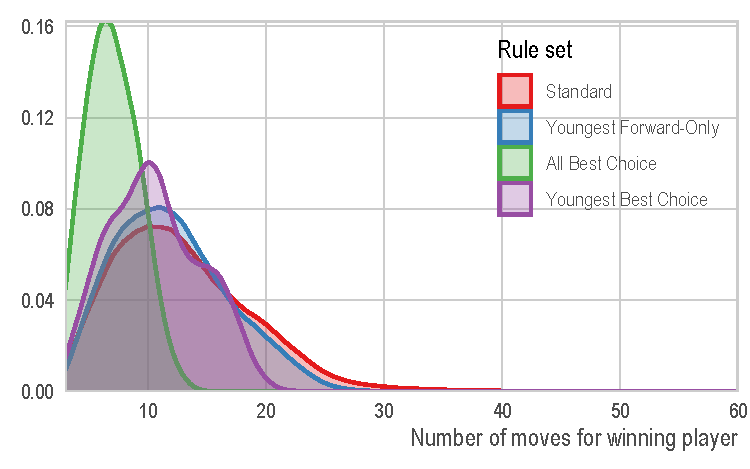
\includegraphics[width=3in]{./../../plots/p_winning_dist.pdf}
    \caption{Distribution of number of moves per game for the winning player.}
    \label{fig:p_winning_dist}
  \end{center}
\end{figure}

\hypertarget{probability-of-player-1-win-as-a-function-of-game-length}{%
\subsection{Probability of Player 1 win as a function of game
length}\label{probability-of-player-1-win-as-a-function-of-game-length}}

In Fig. \ref{fig:p_wins_vs_moves}, we plot the game duration (in number
of moves for the winning player) on the x-axis compared to the
proportion of games won by Player 1 on the y-axis for each rule set
(color). The size of each dot represents the number of simulations.

\begin{figure}
  \begin{center}
    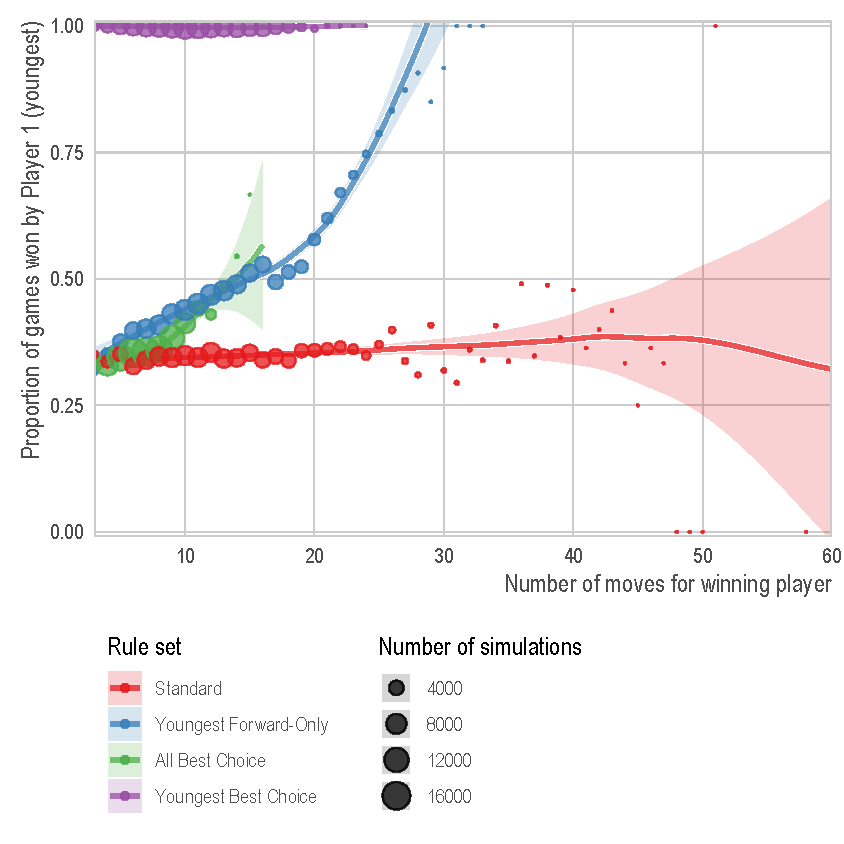
\includegraphics[width=3.25in]{./../../plots/p_wins_vs_moves.pdf}
    \caption{Number of moves required to win (x-axis) relative to the probability of Player 1 winning (y-axis) by rule set (color). The size of each point is the number of simulations. Each line is the loess regression line weighted by the number of simulations.}
    \label{fig:p_wins_vs_moves}
  \end{center}
\end{figure}

As expected, the Standard set shows no correlation with game length.
However, for all restricted game sets, we see that as games get longer,
Player 1 is more likely to win relative to the baseline expected win
percentage of 34.7\%.

\hypertarget{potential-player-locations-quickly-diffuses-over-time}{%
\subsection{Potential player locations quickly diffuses over
time}\label{potential-player-locations-quickly-diffuses-over-time}}

In Fig. \ref{fig:p_positions_by_rules}, we show the potential locations
for Player 1 in the first (top), third (middle), and seventh (bottom)
move for each of the four rule sets. (See the digitized game board as a
stylized grid in For any given bedtime routine, the ideal rule set will
vary. Fig. \ref{fig:p1_board}.)

As expected, in the first move, the location probabilities are identical
across the rule sets. However, diffusion of probabilities across the
board quickly occurs. By the third set, nearly the entire board is a
potential location in the Standard set; however, early squares are less
likely in other sets where backward movement of Player 1 is restricted.
As sets become increasingly restrictive of backward Player 1 movement,
earlier squares are less likely to be available by move 7.

\begin{figure*}
  \begin{center}
    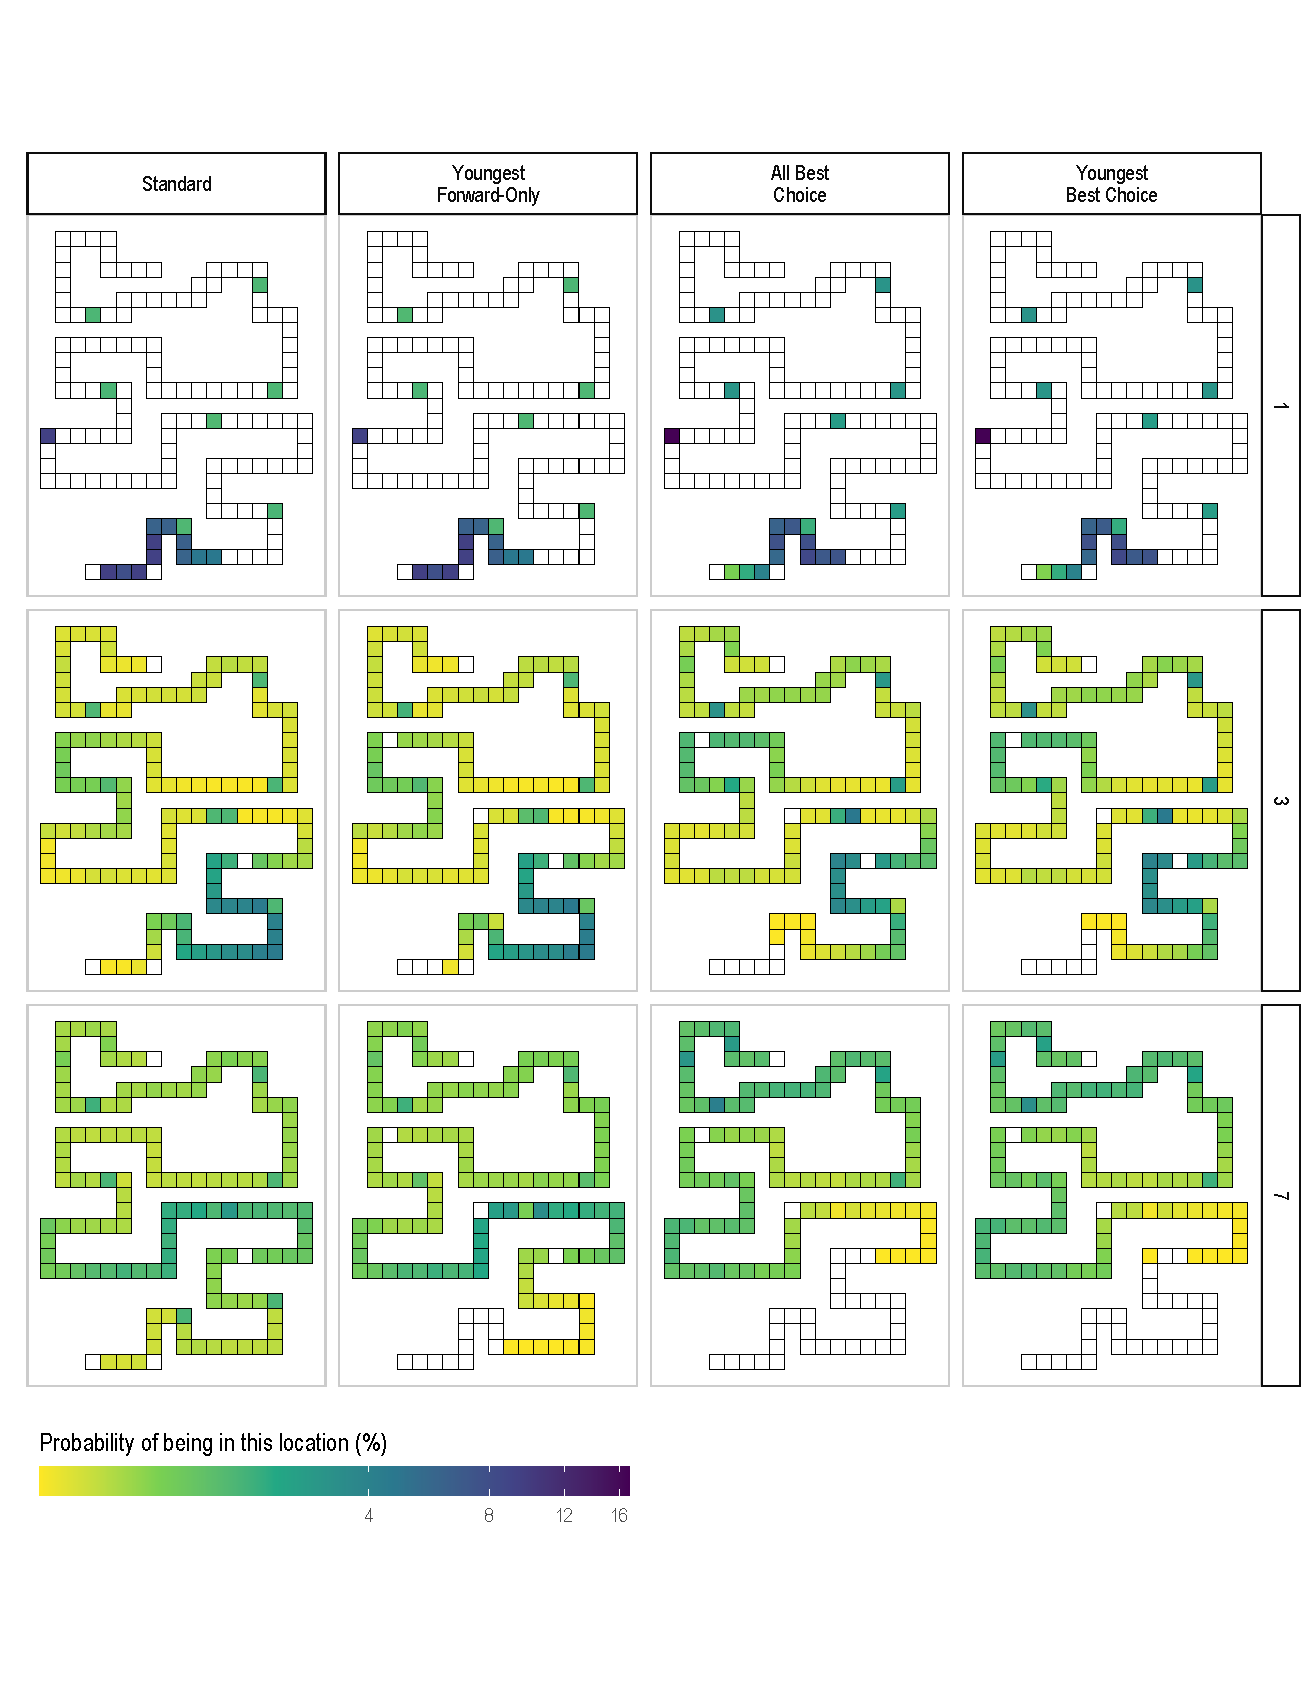
\includegraphics[width=6in]{./../../plots/p_positions_by_rules.pdf}
    \caption{We show the probability of Player 1 board locations for the first (top), third (middle) and seventh (bottom) move by rule sets (columns). In all sets, the first move is identical; however, as backward movement is restricted, the distribution of locations concentrates towards the end of the board with early locations being impossible to return to.}
    \label{fig:p_positions_by_rules}
  \end{center}
\end{figure*}

\hypertarget{different-rule-sets-impact-transition-probabilities}{%
\subsection{Different rule sets impact transition
probabilities}\label{different-rule-sets-impact-transition-probabilities}}

In Fig. \ref{fig:p_transitions}, we plot the probability of transition
from position \(i\) to position \(j\) under each rule set. That is,
given a player is located in position \(i\), what are the probabilities
of transitioning to any other position \(j\). We note, the isolates at
46 and 72 are self-loops due to losing a turn. Horizontal bands
represent the two shortcuts. Vertical bands represent special candy
locations, which can send players forwards or backwards from any board
position.

\begin{figure*}
  \begin{center}
    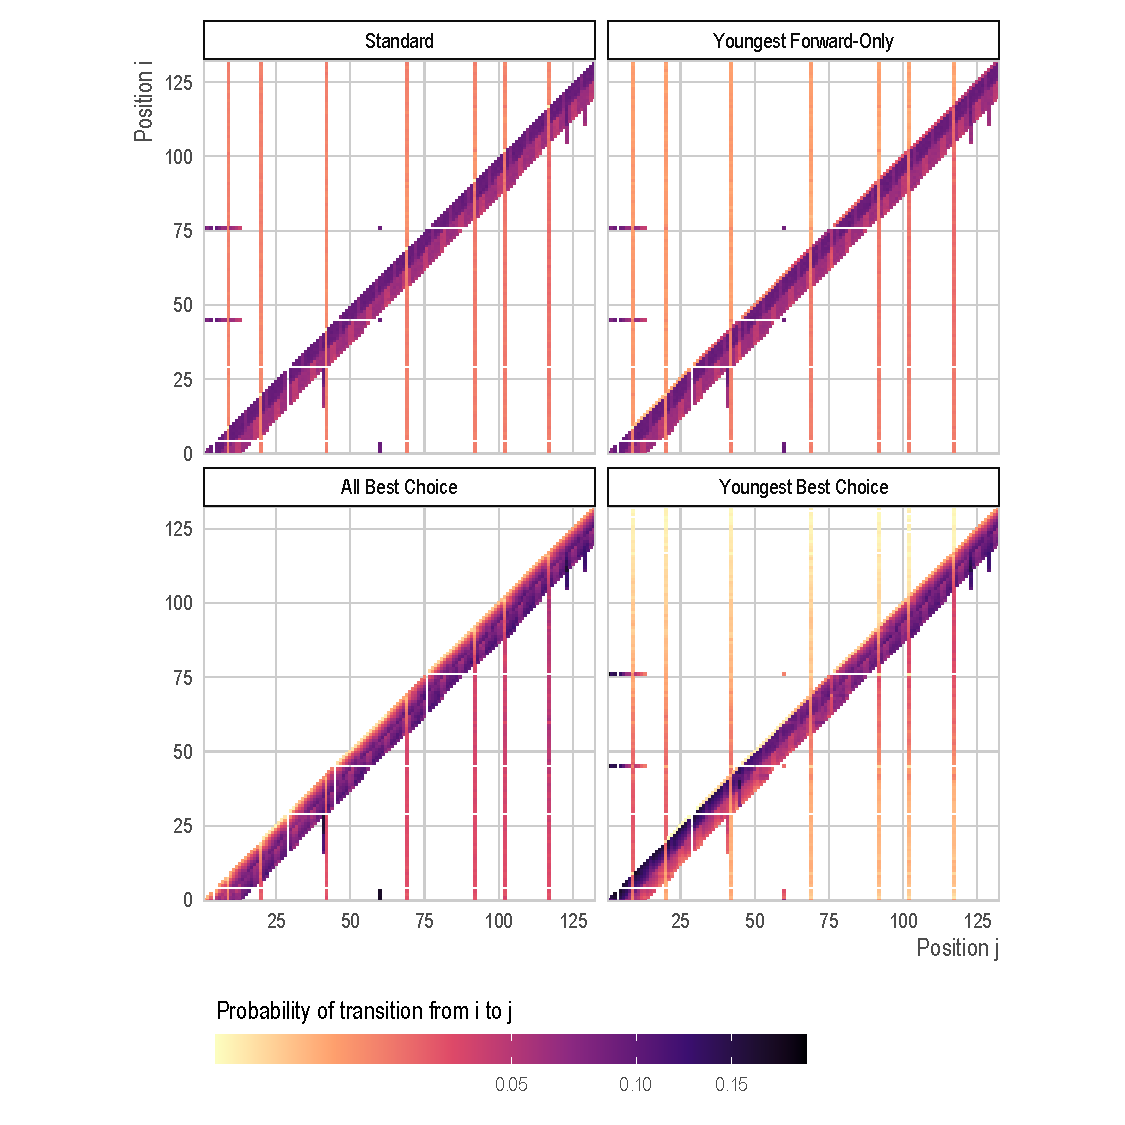
\includegraphics[width=6in]{./../../plots/p_transitions.pdf}
    \caption{For each pair of board positions $i$ and $j$, we show the probability of transitioning to $j$ from $i$ for all 132 board pieces. The isolates at 46 and 72 are self-loops due to losing a turn. Horizontal bands represent the two shortcuts. Vertical bands represent special candy locations, which can send players forwards or backwards from any board position.}
    \label{fig:p_transitions}
  \end{center}
\end{figure*}

\hypertarget{discussion}{%
\section{Discussion}\label{discussion}}

In any given bedtime routine, the ideal rule set will vary. For
Objective 1, maximizing the probability Player 1 wins, the Youngest Best
Choice set is the optimal rule set. Under this set, Player 1 wins over
99.5\% of all games played. For Objective 2, minimizing the game
duration, the the All Best Choice set lasts about half as long as the
Standard set (7 moves vs 13 moves) while also reducing variability in
game duration (SD of 2.2 vs 5.8). While the Youngest Forward-Only set is
not optimal for either objective, it is the most likely to achieve high
compliance by younger players and still provides substantial
improvements over the Standard set.

\hypertarget{ethical-considerations}{%
\subsection{Ethical considerations}\label{ethical-considerations}}

With great power comes great responsibility. Household policymakers must
acknowledge the risk and consequences of employing the implications of
our paper in the real world for prolonged periods of time. As any
academic knows, losing, rejection, and backwards movement are
inevitable, necessary parts of life. Trade-offs between parent mental
health and potentially skewing the world view of young children must be
thoughtfully weighted. We leave this exercise to the reader.

\hypertarget{materials-and-methods}{%
\section{Materials and Methods}\label{materials-and-methods}}

\hypertarget{data}{%
\subsection{Data}\label{data}}

We simulated data using \texttt{R\ 4.0.2}. All code is available in an
online repository. See \textbf{Supplemental Materials}.

\hypertarget{model}{%
\subsection{Model}\label{model}}

We used standard Monte Carlo methods to simulation 100,000 Candy Land
games consisting of three players each under each of the four rule sets.
All code is available in an online repository. See \textbf{Supplemental
Materials}.

\newpage

\hypertarget{supplemental-materials}{%
\section{Supplemental Materials}\label{supplemental-materials}}

\hypertarget{break-down-of-cards}{%
\subsection{Break down of cards}\label{break-down-of-cards}}

There are a total of 64 cards in a standard Candy Land deck. The card
types are single-color, double-color, and special location. For
single-color cards, there are six red, orange, blue, green, and yellow
cards as well as five purple cards. For double-color cards, there are
four red, blue, yellow, and purple cards as well as three orange and
blue cards. There are seven pink cards, each designating a specific
location on the board. In our version of Candy Land (see Fig 3.), the
cards are as follows:

\begin{Shaded}
\begin{Highlighting}[]
\KeywordTok{create_deck}\NormalTok{(}\DataTypeTok{n_decks =} \DecValTok{1}\NormalTok{, }\DataTypeTok{shuffled =} \OtherTok{FALSE}\NormalTok{)}
\end{Highlighting}
\end{Shaded}

\begin{ShadedResult}
\begin{verbatim}
#   [1] "purple_2"      "purple_2"     
#   [3] "purple_2"      "purple_2"     
#   [5] "purple_1"      "purple_1"     
#   [7] "purple_1"      "purple_1"     
#   [9] "purple_1"      "orange_2"     
#  [11] "orange_2"      "orange_2"     
#  [13] "orange_1"      "orange_1"     
#  [15] "orange_1"      "orange_1"     
#  [17] "orange_1"      "orange_1"     
#  [19] "red_2"         "red_2"        
#  [21] "red_2"         "red_2"        
#  [23] "red_1"         "red_1"        
#  [25] "red_1"         "red_1"        
#  [27] "red_1"         "red_1"        
#  [29] "yellow_2"      "yellow_2"     
#  [31] "yellow_2"      "yellow_2"     
#  [33] "yellow_1"      "yellow_1"     
#  [35] "yellow_1"      "yellow_1"     
#  [37] "yellow_1"      "yellow_1"     
#  [39] "green_2"       "green_2"      
#  [41] "green_2"       "green_1"      
#  [43] "green_1"       "green_1"      
#  [45] "green_1"       "green_1"      
#  [47] "green_1"       "blue_2"       
#  [49] "blue_2"        "blue_2"       
#  [51] "blue_2"        "blue_1"       
#  [53] "blue_1"        "blue_1"       
#  [55] "blue_1"        "blue_1"       
#  [57] "blue_1"        "cupcake_1"    
#  [59] "icecream_1"    "gummystar_1"  
#  [61] "gingerbread_1" "lollipop_1"   
#  [63] "popsicle_1"    "chocolate_1"
\end{verbatim}
\end{ShadedResult}

\hypertarget{reproducible-code}{%
\subsection{Reproducible code}\label{reproducible-code}}

All code required to re-run, modify, or inspect this paper is available
online at
\href{http://github.com/mkiang/optimizing_candyland}{\texttt{http://github.com/mkiang/optimizing\_candyland}}.
We note that this code simulates Candy Land under the current
regulations; however, previous iterations of the game had different card
ratios and potentially different board spaces. We provide convenience
functions for changing each as \texttt{create\_deck()} and
\texttt{create\_board()} in the \texttt{./code/utils.R} file.

\begin{figure*}
  \begin{center}
    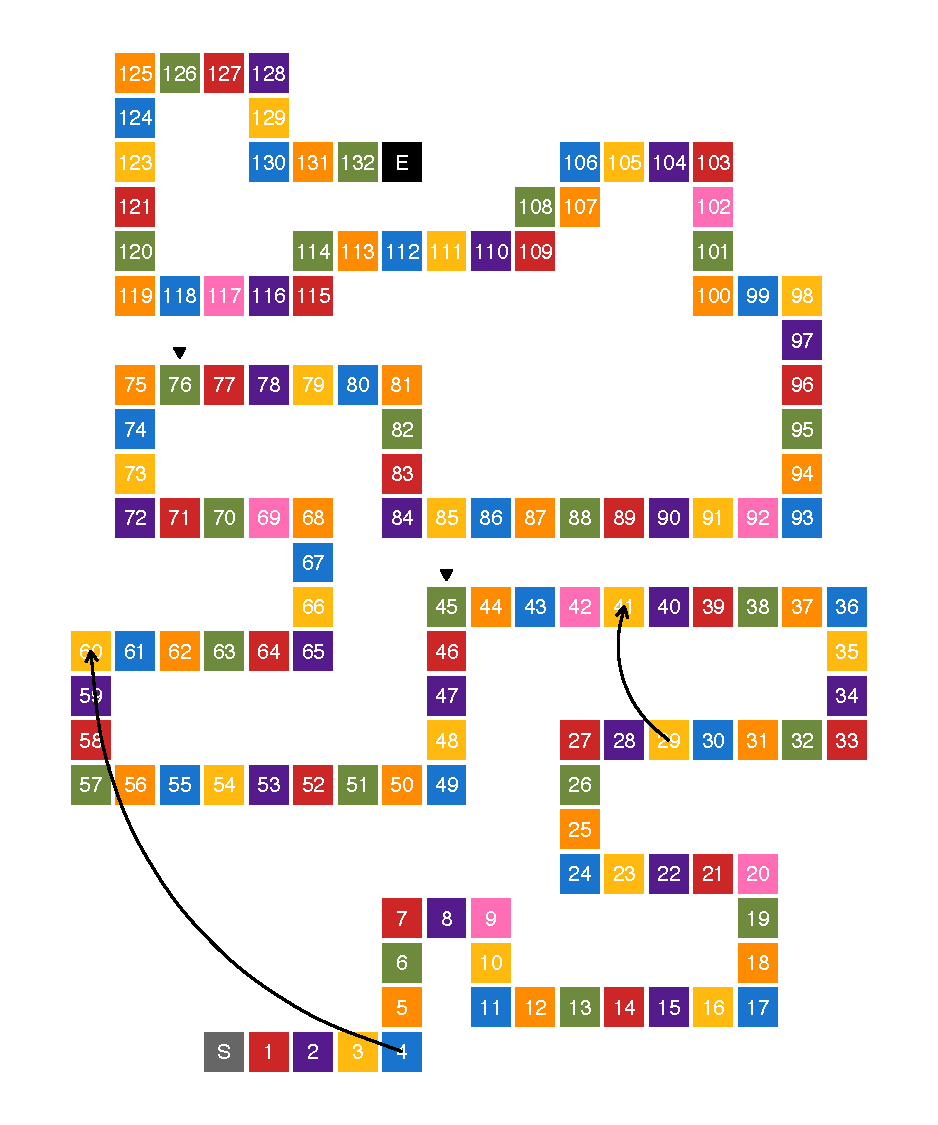
\includegraphics[width=4.5in]{./../../plots/p1_board.pdf}
    \caption{Digitized, stylized Candy Land board. The triangles represent licorice (i.e., lose a turn) squares. The arrows represent paths. Play begins at S in the lower left and ends at E in the top middle.}
    \label{fig:p1_board}
  \end{center}
\end{figure*}

\begin{figure*}
  \begin{center}
    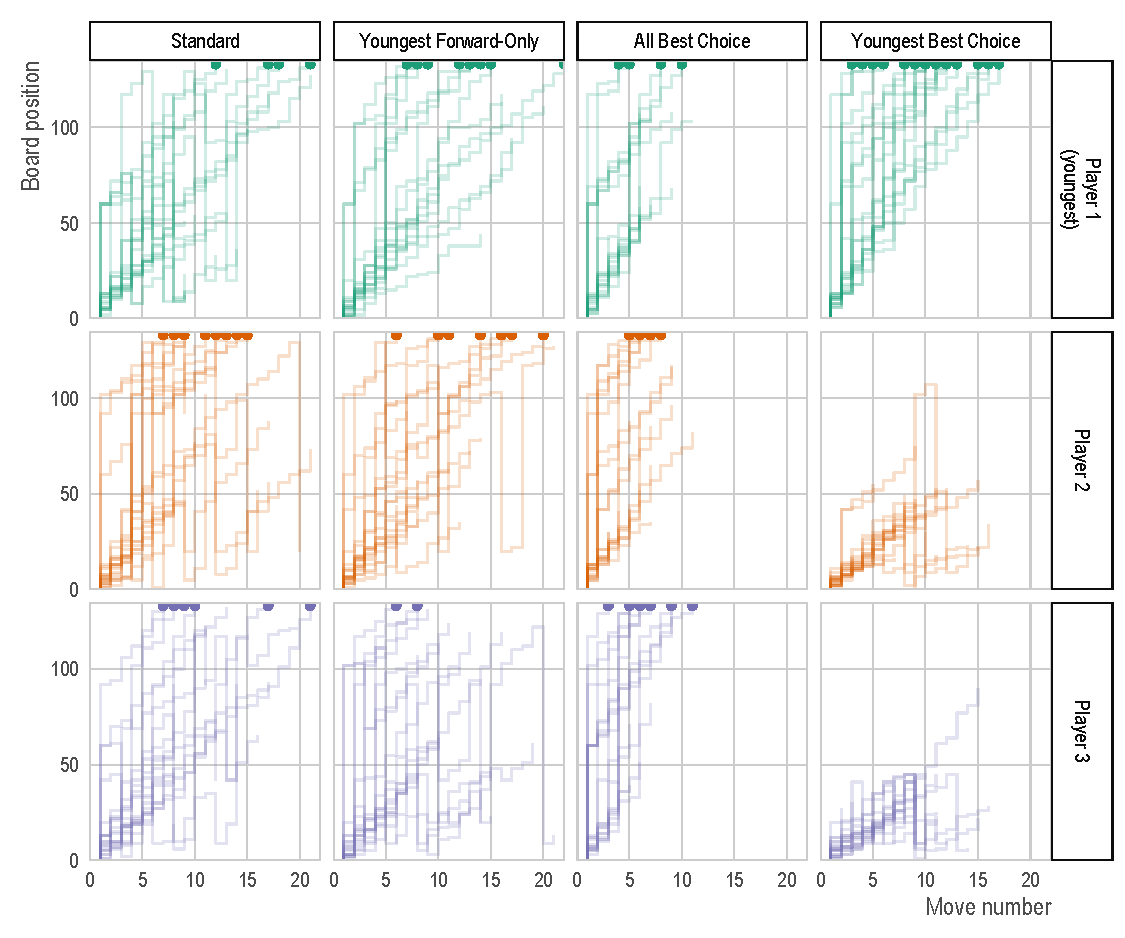
\includegraphics[width=5in]{./../../plots/p_trajectories.pdf}
    \caption{Trajectories for three players (rows) across 20 simulated rounds of Candy Land by rule set (columns). Trajectories that terminated in a victory are marked by a point.}
    \label{fig:p_trajectories}
  \end{center}
\end{figure*}

%\showmatmethods





\end{document}

